\documentclass[runningheads]{llncs}

\usepackage[T1]{fontenc}
\usepackage{graphicx}
\usepackage{xparse} % interval
\usepackage{listings} % code

%%------------------------------------------------
%%------------------------------------------------

\begin{document}
\title{Computer Networks Project: \\ Romanian Railways}

\author{P. Braha\inst{1}\orcidID{0009-0001-3636-2455}}
\authorrunning{P. Braha}
\institute{Alexandru Ioan Cuza University, Iasi IS 700221, Romania
\email{petrubraha@gmail.com}\\
\url{https://github.com/petru-braha}}

\maketitle

\begin{abstract} This work contains an overview of the client-server paradigm offering, to the public transport companies, a concrete (and open source) informational system connected with potential clients. This system provides a service that notifies the consumers about the traveling schedule, the available means of transport (e.g. trains) associated with their time and location, and other related knowledge such as status of departure/arrival and vehicle identification. Any user can report late arrivals, but in a controlled manner such that the misleading records are checked and ignored, if necessary. The application runs concurrently and achieves great communication speed with the customers and good quality of the responses delegated. The security of the system is accomplished by having two different running servers at different locations. If one of them fails, there exists a guaranteed backup. Their communication is not omitted. This paper represents an implementation reference for the field of network programming and management.

\keywords{Server \and Client \and Concurrency \and Transport level \and I/O multiplexing \and Commands \and Threads \and Sockets }
\end{abstract}

%%------------------------------------------------
%%------------------------------------------------

\section{Introduction}

"Romanian Railways" is a project which involves compilation of two programs: one for the server and the other for client(s). It is in a professionally working state when two "server.c" instances are concurrently running indefinitely. One of such instance could manage x number of clients, where $x \in \left[0, 1024\right]$ (this limitation is later disclosed in the forth chapter). 

The current document continues to explain the requirements of such a system, the logic behind it, and the real use cases. Within the next section, a short list of the adopted technologies can be explored. Choosing the right tools will determine the overall quality of the apps. In the third chapter, you may find the structure of the server application, and some illustrations of the routines executed. Following this, additional details, experiments, and observations are analyzed. The advantages and roles of the decisions took regarding the implementation are discussed too. This part creates an opening of the API definitions at application level. The conclusions will summarize my project and propose some scenarios where the "RR application" could be useful.

\subsection{Motivation}

The entire repository is a matter of personal interest for the "Computer Networks" course. Officially, it is known as a laboratory homework, but the main goal is far higher: to be a contribution in practical life. Being encouraged to provide a creative solution, this project was designed.

\section{Applied Technologies}

Three main core objectives were followed in the development: speed, correctness and security. Therefore C programming language was elected because:
\begin{itemize}
    \item it is one of the fastest compiled language 
    \item it supplies network management resources, such as threads and sockets
    \item it delivers simple syntax, yet highly customizable flags and options (very important in the current implementation - see non-blocking calls)
    \item it has all the necessary tools to assure the objectives previously considered; a more advanced language like C++ would add an layer of unnecessary complexity
\end{itemize}

The server has to be concurrent for reasons later argued. To attain this, threads were selected to handle this requirement; they are a multiple-purpose mechanism, as we'll observe in the final composition of the program. Last but not least, the exchange of messages between the customers and the server are realized with sockets through TCP and UDP, transport level protocols.

%%------------------------------------------------
%%------------------------------------------------

\section{Application Structure}

This section covers fundamental information about the internal mechanism of the project, accompanied by a simplified, user-oriented guide. Both parts will consolidate the logic of the operations defined in the server's API. 

\subsection{The order of execution}

The server's program consists of multiple calls and has a rich structure. Because of this, in the next page we will examine a diagram of the core procedures. Breaking down the components of the application(s) into POSIX's standard syntax will form a compacted overview easy to follow along. Doing this also allows us to mark the order of the events: the closer to the top of the figure a function is, the earlier it is being called. Arrows don't necessarily imply succession, they're being used to suggest what to be considered.

\newpage
\begin{figure}[!h]
    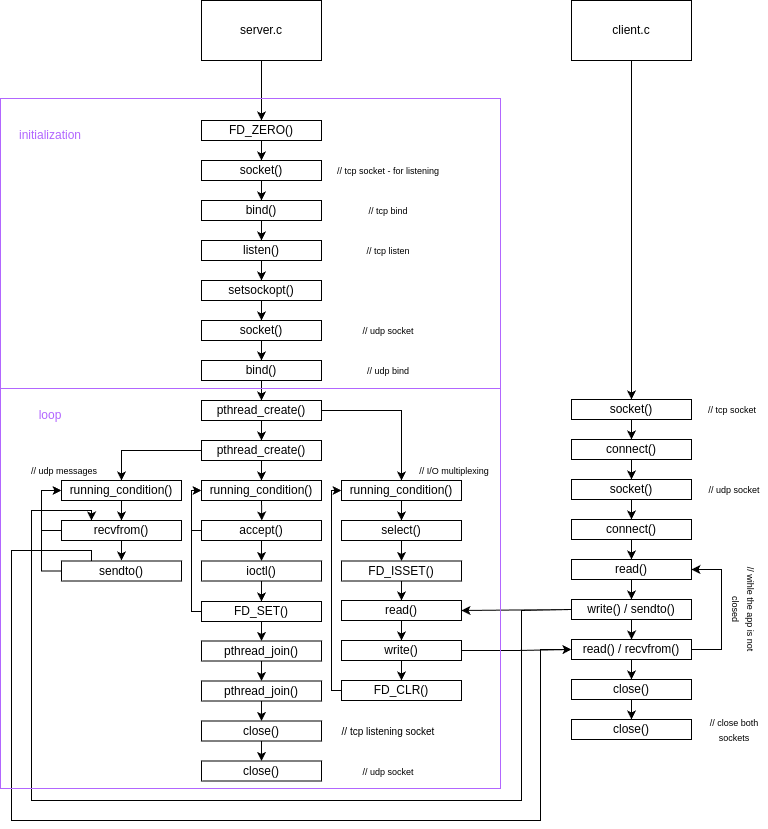
\includegraphics[width=\textwidth]{RR execution diagram.drawio.png}
    \caption{Execution illustration} \label{fig1}
\end{figure}

Before commenting client.c let's focus on the server. This drawing can be splitted into two steps: the initialization stage and the loop. The initialization begins by creating an empty set of socket descriptors - a set which will keep track of the customers. Then, sets-up two non-blocking sockets by linking them with the server's address (setsockopt() and SO\_REUSEADDR are called to avoid distinguishing sockets with other ports). The first socket is the preliminary step of the TCP's three-way handshake (listens for connections) and the second one has a special role (UDP transmissions), explained in the next chapter.

Initialization ends when the process is divided into three threads. Now the server enters in a pseudo-infinite loop. Why pseudo? If an admin logs in, running\_condition() could return false and stop the algorithm. The root thread (the middle one) accepts new connections, while the others organize the data travel. The ioctl() function adds the non-blocking feature to the new clients' sockets, if accepted. They will also be declared in the set initialized earlier. The next thread to be discussed (the one from the right) takes advantage of this set. As we noticed up until now, the socket operations will always be in a non-blocking state, opening the gate for I/O multiplexing. Briefly, clients are treated TCP likewise here, and similarly to this, the last thread (the far left one) has the same purpose but using the UDP communication.

Having this structure of the server is mind follows that every client needs two sockets. Depending on his request type, his message is sent to one of the travel responsible threads using either read() and write(), or sendto() and recvfrom(). The client application also runs in a loop, granting the user to explore live different updates. Note that client's connection-less socket is associated with a connection operation (this article explains more about this phenomenon \cite{udp-connect}).

\subsection{Use case diagram}

\begin{figure}[!h]
    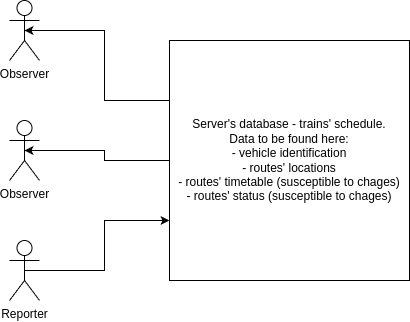
\includegraphics[width=\textwidth]{RR use case diagram.drawio.png}
    \caption{Use case diagram} \label{fig2}
\end{figure}

Keeping the server up allows multiple consumer connections. Those can be categorized as observers or reporters. Reports implies that at least one of their reports was accepted in the system. Everyone receives the demanded data and has the ability to call the report function. But only reporters can impact the schedule.

%%------------------------------------------------
%%------------------------------------------------

\section{Implementation Aspects}

The base of the current code follows the TCP stack model, but with a refined blueprint, outlined in the following subsections. 

\subsection{Concurrency schema}

The server application must be concurrent, otherwise a queue of clients would be formed and their requests will be delivered slowly. The following list of strategies were evaluated in our build:
\begin{itemize}
    \item pre-forking
    \item pre-threading
    \item fork per client
    \item thread per client
\end{itemize}

Using threads over child processes is due to their "shared memory" character (please also note: \cite{fork-vs-thread}). Even if a child process is "copy on write" optimized, it is not the best choice for a long-term running server which frequently updates all of the data. 

What about the "pre-threading"? Approaching this requires to fix a specific number of threads, say $x$, which could be overwhelm by $x + 1$ clients. This fault could be countered with adding threads for the exceeding number of customers. Theoretically speaking, this would represent the obvious choice if the security means are ignored. As previously stated, security is attained using two different servers which have different hardware specifications. The constant number of threads has to adapt for the machines with different components, acknowledging the fact that in the future it is intended to increase this security factor by adding another running instances of the server.

So, the final configuration is a hardware-portable combination of the second and forth approaches. The server starts with three threads. Let the basic iterative TCP server be our guide for now (an example can be viewed here: \cite{course} - week 5). It has to accept connections, to manage descriptors, and also to send data. Wouldn't it be faster to run these concurrently? The initial three threads of the server precisely solves these tasks. One thread takes care of the connections, another checks which customers are ready to be dealt with, and the last one's role is to provide a gateway for connection-less requests.

\subsection{Transport protocol}

The transport layer uses a combination of TCP and UDP, where their advantages were exploited for the appropriate situations in the code.

The TCP protocol is used for the commands that influence the server's data. Being a secure protocol, TCP provides acknowledgments for all the transmitted messages. However, it implies an increased amount of time, which proposes the usage of the UDP protocol. TCP is a robust mechanism which assures correctness of transmissions, which is mandatory for clients' reports. But, in cases of simpler queries, it is preferred a faster communication. If the communication fails, it can be simply readdressed by the consumer.

Wrong outputs were avoided. If nothing is received at one end the clients has to resend the same query. If something wrong is received at server's end, it is capable of interpreting and remodel the request. The only way to check if an output is correct on the customer's end, is to resend the query.

Briefly, the clients use TCP when sending requests to change the trains' schedule, and UDP for information retrieval.

\subsection{I/O Multiplexing}

This topic improves further the speed of the client-server correspondence. The select() primitive with unblocking I/O operations is considered to bring exceptional results, (accordingly to \cite{non-block-select} and \cite{course} - week 7). What is better than an iterative server with I/O multiplexing? A concurrent one, which uses the same principle.

\subsection{Innovative scores}

Inclusion of an administrator login is considered a simple, yet useful contribution. Instead of manually crashing the server, an admin could insert a key into a specific file, monitored by the application. If that key is "1" everything will work as planned - the system will be online. In the opposite case, servers automatically shuts down, avoiding memory leaks and errors.

One other interesting feature is the second end of the server. By default, the initialization of the data is done at 10.100.0.30 - the primary instance of the server - which is always online. The second end is being held by my personal computer, and instead of manually copying the data files, it communicates with the primary instance. Doing so we're keeping a ready-to-replace and functional copy.

\subsection{Definitions}

In the succeeding lines we'll describe the dialect used in the application protocol. 

\begin{itemize}
    \item route = an itinerary is from point A to point B and no other points. In memory it is composed of an id\_train, two location points, two time delimitations and a status field, forming a rr\_route struct.

    \item locations types: departures, arrivals. They are being recognized as integers.

    \item estimated times = initial times defined by the generated schedule
    \item confirmed times = estimated times +/- delays. A clear distinction is made between "estimated" and "confirmed". The former has an information initializing character, while the second emphasizes that the information is a subject to modifications.
    
    \item times types: confirmed departure time, estimated departure time, confirmed arrival time, estimated arrival time.
    
    \item status of a train has two fields - each indicates whether it has left the departure location or arrived at destination. Both will be as a boolean variable int the rr\_status struct.
\end{itemize}

Server's activity consists of:
\begin{itemize}
    \item sending data to clients
    \item reading data from XML files
    \item receiving reports from clients
    \item updating the data (delays, arrival estimation) based on the reports
\end{itemize}

The time of the application is the current Romania's time (GMT+2). It is considered that the trains that are late for more than three hours are defect.

Client's application builds the final string messages based on the data returned by the server. 

%%------------------------------------------------
%%------------------------------------------------

\subsection{Application protocol}

\begin{enumerate}
   \item \begin{itemize} \item NAME: routes - the complete trains' schedule for the present day
            \item SYNOPSIS: struct rr\_route* routes(int location\_departure, int location\_arrival)  
            \item DESCRIPTION: Receives as parameters the desired path of the traveler and iterates through the routes for matching location settings. Not finding any such itinerary is considered an failure.
            \item RETURN VALUE: On success, routes() returns a pointer to a block of memory being composed of the schedule's data. On failure, it returns a NULL-pointer.
            \item NOTES: If one of the descriptors is invalid the function fails. 
            \item EXAMPLES: \begin{lstlisting}[language=C++]
    #define IASI 101
    #define BUCHAREST 100
    struct rr_route* it = routes(IASI, BUCHAREST);
    while(it) {
        // server sends the data 
        write(sd, *it, sizeof(struct rr_route));
        it++; 
    }
            \end{lstlisting}
            \vspace{0.3cm}
   \end{itemize}
   
   \item \begin{itemize} \item NAME: departures - routes and trains in the next hour
            \item SYNOPSIS: struct rr\_route* departures(int location\_departure)  
            \item DESCRIPTION: It iterates through  all the routes and checks the departure locations field for the integer provided. If found, it returns a not NULL-pointer. 
            \item RETURN VALUE: On success, departures() returns a pointer to a block of memory - a list of the routes matching the argument. On failure, it returns a NULL-pointer.
            \item NOTES: the extra data is filtered out by the client's application
            \vspace{0.3cm}
   \end{itemize}
   
   \item \begin{itemize} \item NAME: arrivals - routes and trains in the next hour
            \item SYNOPSIS: struct rr\_route* arrivals(int location\_arrival)
            \item DESCRIPTION: It iterates through  all the routes and checks the arrival locations field for the integer provided. If found, it returns a not NULL-pointer. 
            \item RETURN VALUE: On success, arrival() returns a pointer to a block of memory - a list of the routes matching the argument. On failure, it returns a NULL-pointer.
            \item NOTES: the extra data is filtered out by the client's application
            \vspace{0.3cm}
   \end{itemize}
   
   \item \begin{itemize} \item NAME: report - sends requests to update the schedule and related buffers.
            \item SYNOPSIS: void report(int id\_train, int minutes)  
            \item DESCRIPTION: It iterates through  all the routes to find the id of the train. If it is found, the status is checked and set accordingly.
            \item ERRORS: \begin{itemize}
                \item RR\_ERR\_REP0 - the id\_train is an invalid id. 
                \item RR\_ERR\_REP1 - the id\_train is marked as arrived. 
                \item RR\_ERR\_REP2 - the id\_train is not marked as left.
                \item RR\_ERR\_REP3 - more than 180 minutes are reported.
            \end{itemize}
            \item NOTES: It follows the TCP transmission type.
            \item EXAMPLES: 
    // let 100 be an arrived train, 101 a train marked as left but not arrived, 102 a train not marked as left  
    \begin{lstlisting}[language=C++]
    report(100, 5);     // fails
    report(101, 5);     // works
    report(101, 181);   // marked as defect
    report(102, 15);    // fails
            \end{lstlisting}
            \vspace{0.3cm}
   \end{itemize}
   
   \item \begin{itemize} \item NAME: quit - allows the consumer to close the application
            \item SYNOPSIS: void quit()  
            \item DESCRIPTION: This function is definite in closing the communication with the server. Once typed the application will close.
            \item NOTES: It follows the TCP transmission type.
            
            If the server shuts down before the client, quit() saves the user from any potential bug.
   \end{itemize}
\end{enumerate}

%%------------------------------------------------
%%------------------------------------------------

\section{Conclusions}

Finally, this work concludes as a reference for the applied principles of network management. It showcases a fast, correct and secure implementation that uses a lot of different approaches to maximize these goals. To increase speed it was utilized: a concurrent server, UDP and a hybridized TCP with I/0 multiplexing. The durability is maintained by the second running server.

\begin{credits}
    \subsubsection{\ackname} This open-source project has no financial support. Improvements and updates are expected only for the following month.
    \subsubsection{\discintname}
    There are no competing interests to declare, that could be relevant to the content of this article.
    \end{credits}
    

%%------------------------------------------------
%%------------------------------------------------

\begin{thebibliography}{8}

\bibitem{diagram-site} "draw.io". Diagram drawing tool. \\ \url{https://app.diagrams.net/}

\bibitem{udp-connect}
T. Gavrichenkov. "Can you bind() and connect() both ends of a UDP connection". Stack Overflow. Accessed on 29.11.2024. \\
\url{https://stackoverflow.com/questions/9741392/can-you-bind-and-connect-both-ends-of-a-udp-connection}

\bibitem{fork-vs-thread} Sysel, Martin. "A comparison of processes and threads creation". Software Engineering Perspectives in Intelligent Systems: Proceedings of 4th Computational Methods in Systems and Software 2020, Vol. 1 4. Springer International Publishing, 2020. \\ 
\doi{10.1007/978-3-030-63322-6_85}

\bibitem{course}
L. Alboaie, A. Panu. "Computer Networks" - course page. Alexandru Ioan Cuza University, 2024. \\
\url{https://edu.info.uaic.ro/computer-networks/index.php}

\bibitem{non-block-select} Stevens, W. Richard, Andrew M. Rudoff, and Bill Fenner. Unix network programming volume 1: the sockets networking API. Vol. 3. Boston: Addison-Wesley Professional, 2003.

\bibitem{ibm} "Example: Nonblocking I/O and select()". IBM's company. Accessed on 26.11.2024. \\
\url{https://www.ibm.com/docs/en/i/7.3?topic=designs-example-nonblocking-io-select}

\end{thebibliography}
\end{document}
